\subsection{Gravity}
$M_*$ - central mass. $m \ll M_*$. Force of gravity is $\vec{F} = -\hat{r}\frac{GM_*}{r^2}m$ and gravitational energy $U_g = - \frac{GM_*m}{r}$.

Total energy is $$E = \frac{1}{2}mv^2+\left( -\frac{GM_*m}{r} \right)$$
where $v = v_r\hat{r}+v_\theta\hat{\theta}$, when $v_\theta = \frac{J}{mr}$ since radial velocity doesn't affects angular momentum. Substituting:

$$E=\frac{1}{2}m\dot{r}^2+\frac{1}{2}m\left( \frac{J}{mr}\right)^2 -\frac{GM_*m}{r} = \frac{1}{2}m\dot{r}^2+\underbrace{\frac{J^2}{2mr^2}}_{\parbox{2cm}{\centering \scriptsize centrifugal potential}} -\frac{GM_*m}{r}$$

Define effective potential which depends only on $r$ and not on $\theta$: $U_{eff} = \frac{J^2}{2mr^2} - \frac{GM_*m}{r}$. So:

$$E = \frac{1}{2}m\dot{r}^2 + U_{eff}(r)$$

This equation is only in one dimension $r$ and not describes all the trajectory.

\paragraph{Different trajectories of bodies} Kinetic energy is positive to the right of the blue line, which is total potential, and equals to 0 (i.e. $\dot{r}=0$) at the line:
\begin{center}
	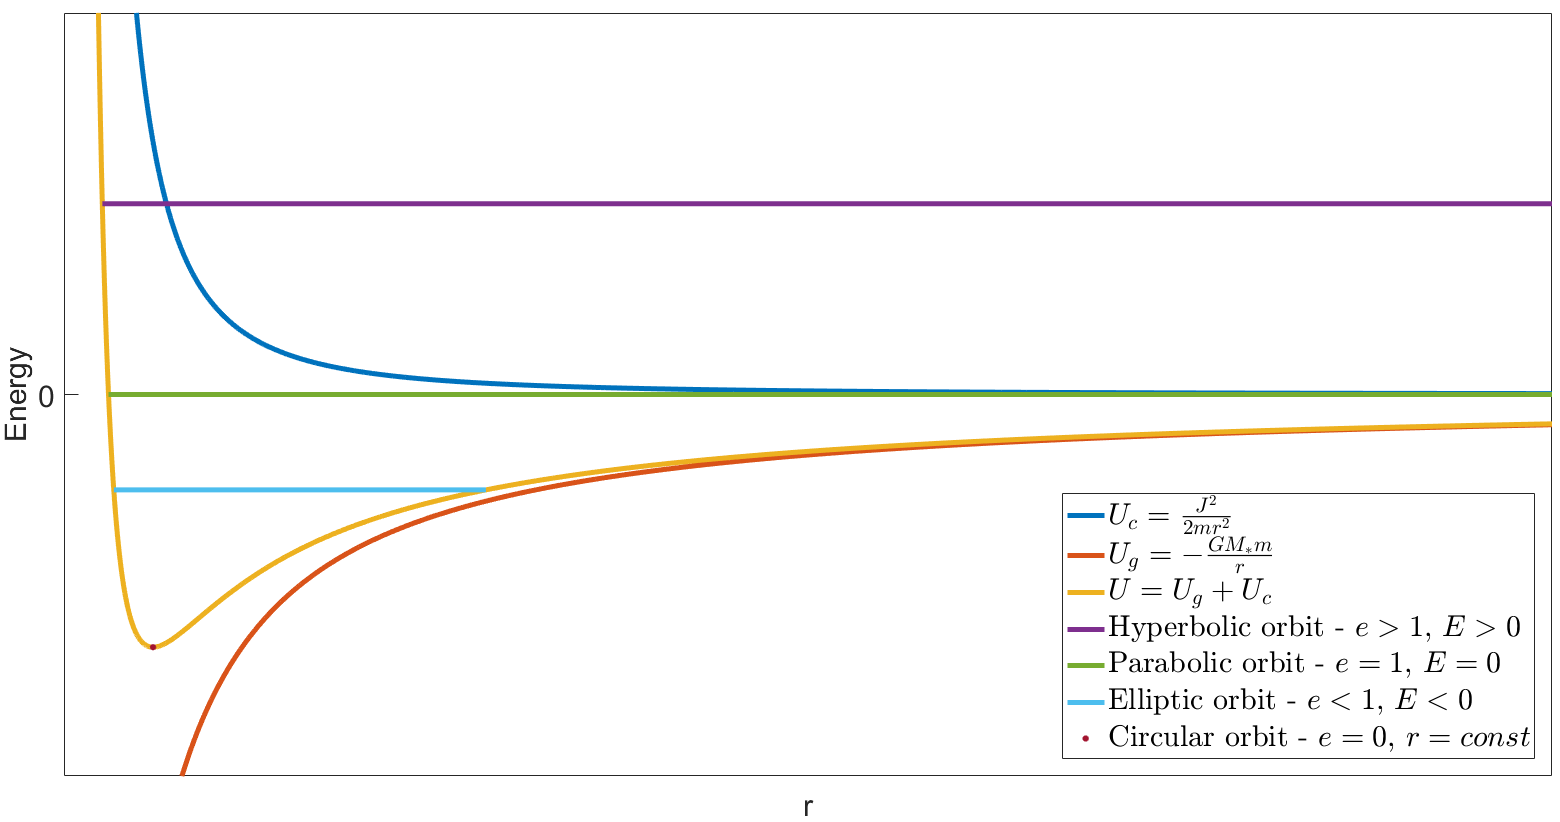
\includegraphics[width=\linewidth]{./lect15/pic1.png}
\end{center}
\begin{center}	
	\includesvg[eps,svgpath = lect15/,width=0.7\linewidth]{pic2}
\end{center}

\textbf{Note:} Hyperbolic orbit works also with repelling, for example electrical force. 
\paragraph{Circular orbit} $\dot{r} = 0$ and $\vec{v} = v_\theta \hat{\theta}$.

Centrifugal force equals to gravitational force:

$$m \frac{v^2}{r} = \frac{GM_*m}{r^2}$$
Velocity is $v = \sqrt{\frac{GM_*}{r}}$, angular velocity is $\omega = \frac{v}{r} = \sqrt{\frac{GM_*}{r^3}}$ and cycle time is $T=\frac{2\pi}{\omega} = \frac{2\pi r}{v} = 2\pi \cdot \frac{r^{\frac{3}{2}}}{\sqrt{GM_*}}$

\paragraph{Kepler's laws}
\begin{enumerate}
	\item  The orbit of a planet is an ellipse with the Sun at one of the two foci.
	\item A line segment joining a planet and the Sun sweeps out equal areas during equal intervals of time.
	\item The square of the orbital period of a planet is proportional to the cube of the semi-major axis of its orbit.
	
\end{enumerate}

\begin{center}
	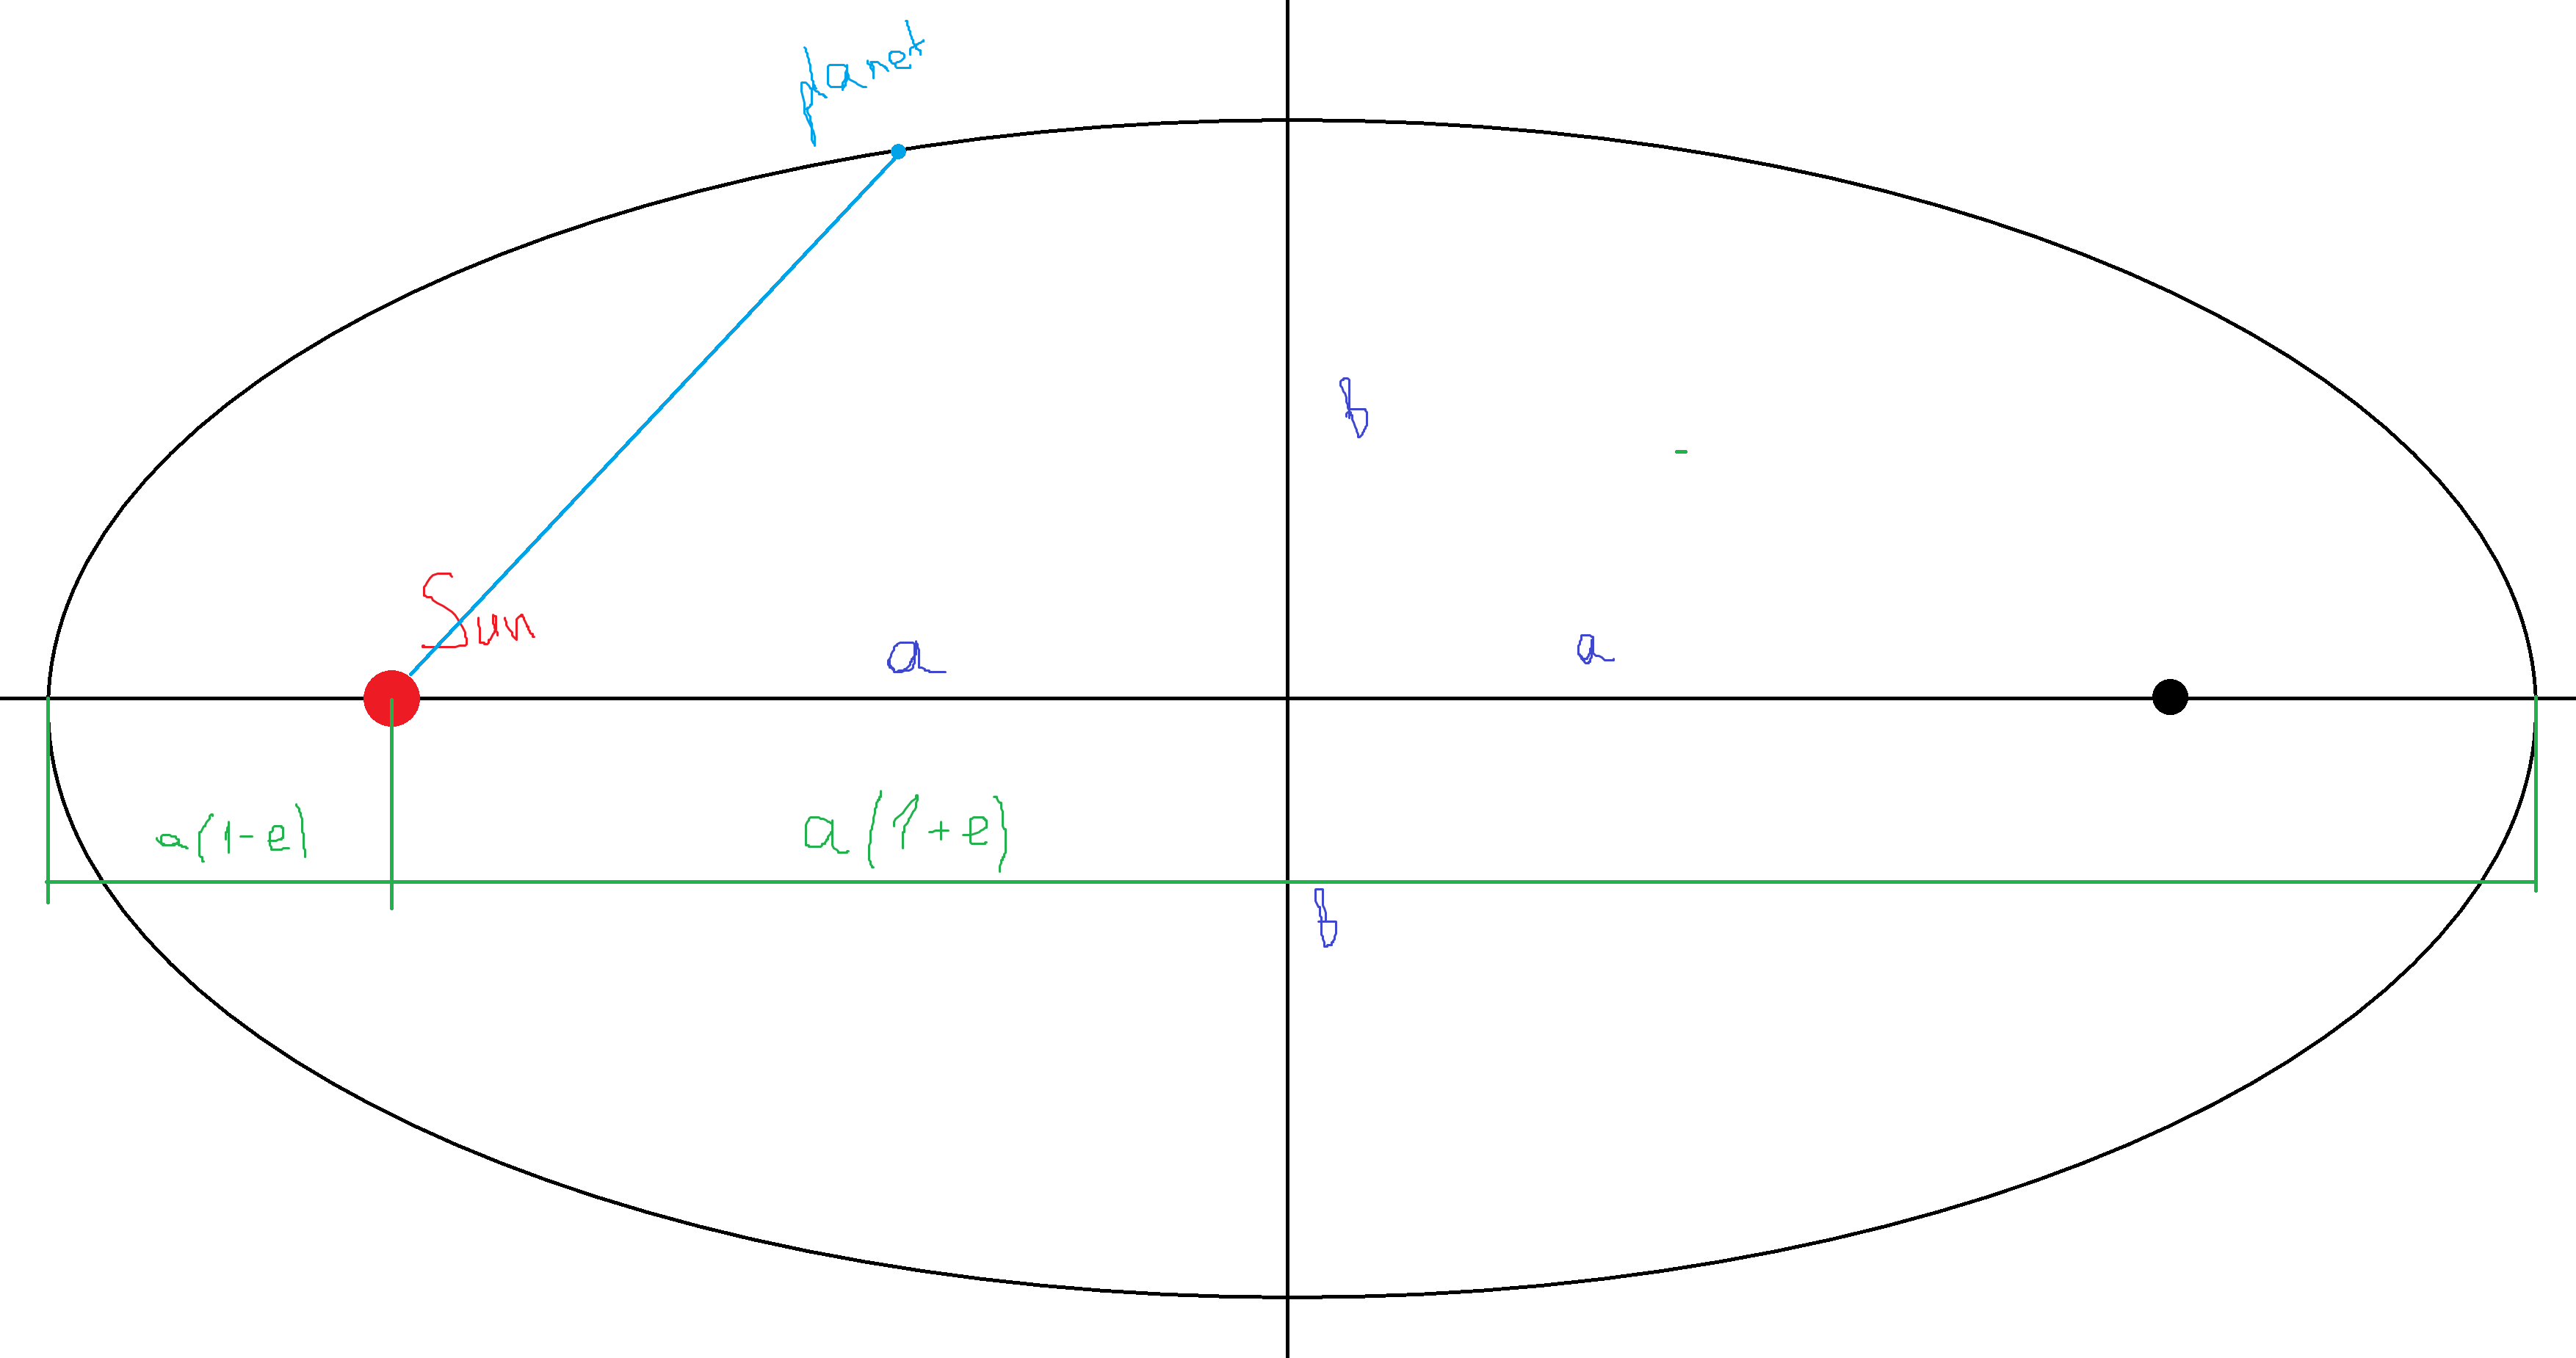
\includegraphics[width=\linewidth]{./lect15/pic3.png}
\end{center}

$b = a\sqrt{1-e^2}$.

Ellipse equation is $$r = \frac{a\left( 1-e^2 \right)}{1-e\cos \theta}$$

\paragraph{Physical solution} of movement of $m$ around $M_*$.
From second law:
$$m\vec{a} = \vec{F}$$

Force is $\vec{F}  =-\hat{r}\frac{GM_*m}{r^2}$ and acceleration $\vec{a} = \left( \ddot{r} - r\dot{\theta}^2 \right)\hat{r} + \frac{1}{r}\frac{d}{dt}\left( r^2\dot{\theta} \right)\hat{\theta}$

Movement equation in direction $\hat{\theta}$:

$$m\frac{1}{r}\frac{d}{dt}\left( r^2 \dot{\theta} \right) = F_\theta = 0$$
$$\frac{d}{dt}\left( r^2 \dot{\theta} \right) = 0$$
$$r^2 \dot{\theta} = const$$

Multiplying by $m$:

$$mr^2 \dot{\theta} = const  =J$$

Since $r\dot{\theta} = r \frac{d\theta}{dt} = v_\theta$:

$J=mrv_\theta=const$

Movement equation in direction $\hat{r}$:

$$m\left( \ddot{r} - r\dot{\theta}^2 \right) = -\frac{GM_*m}{r^2}$$

Substituting $\dot{\theta} = \frac{J}{mr^2}$:

$$\ddot{r} - r\frac{J^2}{m^2r^4} = -\frac{GM_*}{r^2}$$

We get the equation:

$$\frac{J^2}{m^2r^4}\left[ \frac{d^2r}{d\theta^2} - \frac{2}{r}\left( \frac{dr}{d\theta} \right)^2 \right] - r\frac{J^2}{m^2r^4} = -\frac{GM_*}{r^2}$$

The solution of this differential equation is:

\begin{align*}
\frac{1}{r} = \frac{GM_*}{\left( \frac{J}{m} \right)^2} \left[ 1 - \left( 1+ \frac{2\left( \frac{E}{m} \right)\left( \frac{J}{m} \right)^2}{G^2M_*^2} \right)^{\frac{1}{2}}  \cos \theta \right]
\end{align*}

When eccentricity:

$$e=\left[ 1+ \frac{2\left( \frac{E}{m} \right)\left( \frac{J}{m} \right)^2}{G^2M_*^2} \right]^{\frac{1}{2}}$$ 